% Template for Cogsci submission with R Markdown

% Stuff changed from original Markdown PLOS Template
\documentclass[10pt, letterpaper]{article}

\usepackage{cogsci}
\usepackage{pslatex}
\usepackage{float}
\usepackage{caption}

% amsmath package, useful for mathematical formulas
\usepackage{amsmath}

% amssymb package, useful for mathematical symbols
\usepackage{amssymb}

% hyperref package, useful for hyperlinks
\usepackage{hyperref}

% graphicx package, useful for including eps and pdf graphics
% include graphics with the command \includegraphics
\usepackage{graphicx}

% Sweave(-like)
\usepackage{fancyvrb}
\DefineVerbatimEnvironment{Sinput}{Verbatim}{fontshape=sl}
\DefineVerbatimEnvironment{Soutput}{Verbatim}{}
\DefineVerbatimEnvironment{Scode}{Verbatim}{fontshape=sl}
\newenvironment{Schunk}{}{}
\DefineVerbatimEnvironment{Code}{Verbatim}{}
\DefineVerbatimEnvironment{CodeInput}{Verbatim}{fontshape=sl}
\DefineVerbatimEnvironment{CodeOutput}{Verbatim}{}
\newenvironment{CodeChunk}{}{}

% cite package, to clean up citations in the main text. Do not remove.
\usepackage{cite}

\usepackage{color}

% Use doublespacing - comment out for single spacing
%\usepackage{setspace}
%\doublespacing


% % Text layout
% \topmargin 0.0cm
% \oddsidemargin 0.5cm
% \evensidemargin 0.5cm
% \textwidth 16cm
% \textheight 21cm

\title{Conceptual and prosodic cues in child-directed speech can help children
learn the meaning of disjunction}


\author{{\large \bf Masoud Jasbi} \\ \texttt{masoudj@stanford.edu} \\ Department of Linguistics \\ Stanford University \And {\large \bf Akshay Jaggi} \\ \texttt{ajaggi@stanford.edu} \\ Department of Linguistics \\ Stanford University \And {\large \bf Michael C. Frank} \\ \texttt{mcfrank@stanford.edu} \\ Department of Psychology \\ Stanford University }

\begin{document}

\maketitle

\begin{abstract}
Current theories of word learning focus on cues and mechanisms that help
children's acquisition of open-class words such as nouns and verbs.
Little is understood about the role of input in children's acquisition
of closed-class words such as articles and connectives. This paper
investigates the cues in child-directed speech that can help the
interpretation and acquisition of the connective \emph{or}. Study 1 uses
a large corpus of parent-child interactions to show that despite low
occurance of \emph{or} in child-directed speech, children quickly reach
the adult level of production for this word by age 4. Study 2 uses
annotations on a subset of parent-child interactions to show that
disjunctions in child-directed speech are accompanied by reliable cues
to the correct interpretation (exclusive vs.~inclusive). We present a
computational model that learns from a handful of annotated examples to
correctly predict the interpretation of a disjuntion. These studies
suggest that reliable cues in child-directed speech can assist rapid
acquisition of functional categories such as disjunction words.

\textbf{Keywords:}
language acquisition; word learning; logical words; conjunction,
disjunction.
\end{abstract}

\section{Introduction}\label{introduction}

When we think of words, we often think of nouns like \emph{cat},
adjectives like \emph{red}, or verbs like \emph{run}. These classes of
words - called \textbf{content words} - have thousands of members and
constantly add new ones like \emph{Google}, \emph{crunk}, or
\emph{chillax}. Their meanings often refer to concrete and tangible
entities or events in the world. This is not the case for
\textbf{function words} like \emph{and}, \emph{or}, \emph{of}, and
\emph{the}. Functional classes have few members and rarely accept new
ones. Their meanings are highly abstract and provide the glue that holds
content words together to form complete thoughts. These properties make
function words challenging for theories of word learning.

Word learning is often construed as the process of isolating a word
form, selecting a meaning from a set of candidate meanings, and mapping
the word form to the selected meaning (Clark, 1995). While there has
been a lot of research on cues and constraints that assist children in
selecting the right meaning for content words, very little is known
about the cues that help children's learning of functional meaning. This
study makes the initial steps in discovering such cues by investigating
the disjunction word \emph{or} in parents' and children's speech.

The word \emph{or} has long been a lab rat in linguistics and language
acquisition. This interest in \emph{or} is mainly due to its close
connection to logical disjunciton. In formal logics, there are two types
of disjunction: inclusive and exclusive. An \textbf{inclusive
disjunction} such as ``A \(\vee\) B'' is true when either A, B, or both
are true. An \textbf{exclusive disjunction} such as ``A \(\oplus\) B''
is true only when A or B is true but not both. The linguistic connective
\emph{or} can receive an inclusive interpretation like ``A \(\vee\) B''
or an exclusive one like ``A \(\oplus\) B''. For example, a waitor may
ask if you would like something to eat or drink, not excluding the
possibility that you would like both. However, the waitor may later ask
if you would like to see the dessert menu or have the cheque, suggesting
that you should chose one or the other.

A large body of research in formal semantics and pragmatics seeks to
specify the meaning of \emph{or} and factors that determine its
interpreation as inclusive and exclusive. Grice (1975) argued that the
core meaning of \emph{or} is inclusive disjunction. The exclusive
interpretation is the result of modifying this inclusive meaning by
factors external to \emph{or} itself. He suggested that upon hearing ``A
or B'', we may exclude the possibility of both A and B being true simply
because we reason that the speaker could have used the connective
\emph{and} instead of \emph{or}. Therefore, the exclusive interpretation
is the result of this pragmatic reasoning on the speaker's choice of
\emph{or} instead of \emph{and} and not part of the meaning of \emph{or}
itself. Geurts (2006) argued that in many cases, exclusive
interpretations stem from the inconsistent meaning of the options. For
example, ``to be or not to be'' is exclusive simply because one cannot
both be and not be! In an experimental study, Pruitt \& Roelofsen (2013)
showed that in questions, exclusive interpretations are the result of a
rise-fall intonation. In short, while the meaning of \emph{or} itself is
inclusive, the situation where both options are true may be excluded by
pragmatic reasoning, inconsistent options, or a rise-fall intonation.

\begin{CodeChunk}
\begin{figure}[b]

{\centering 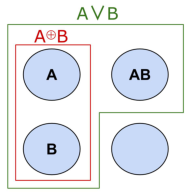
\includegraphics{figs/aorb-1} 

}

\caption[Inclusive disjunction (A$\vee$B) is true in situations where A, B, or both AB are true]{Inclusive disjunction (A$\vee$B) is true in situations where A, B, or both AB are true. Exclusive disjunction (A$\oplus$B) is true in situations where only A or only B is true.}\label{fig:aorb}
\end{figure}
\end{CodeChunk}

Research in formal semantics and pragmatics raises a developmental
question: how do children learn the meaning of \emph{or} given the
ambiguity it can give rise to? To answer this, Morris (2008)
investigated instances of \emph{and} and \emph{or} in parents' and
children's speech. He found that \emph{and} occurs about 3 times every
100 utterances in the speech of parents while \emph{or} occurs only once
or twice every 400 utterances. More importantly, children reach the
adult level of production for \emph{and} relatively quickly and around
the age 3 but their productions of \emph{or} do not reach the adult
level in the first five years. He also found that the majority of
\emph{or} examples children hear (75-80\%) and produce (\%90) have an
exclusive interpretation. Based on these findings, he concluded that
children's acquisition of \emph{or} is slow and they understand its
meaning as exclusive before they add the inclusive meaning to their
repertoire.

However, experimental studies find that children between the ages 3 to 5
interpret \emph{or} as inclusive disjunction (Chierchia, Crain, Guasti,
Gualmini, \& Meroni, 2001; Crain, 2012; Jasbi \& Frank, 2016). This is
surprising given Morris (2008)'s finding that the majority of \emph{or}
examples children hear and produce are exclusive. How do children learn
the inclusive meaning of \emph{or} if they rarely hear it? Crain (2012)
suggested that children rely on an innate universal principle that
disjunction words must not be mapped onto exclusive meanings. In other
words, in hearing a connective form, children consider inclusive
disjunction (A \(\vee\) B) as a viable meaning and not exclusive
disjunction (A \(\oplus\) B).

Here we present two studies that suggest children can rapidly learn the
interpretation of disjunction from the conceptual and prosodic cues that
accompany it in child-directed speech. In study 1, we use a large corpus
of parent-child interactions to show that both \emph{and} and \emph{or}
appear relatively quickly in children's speech and reach the adult rate
of production by the age 4. In study 2, we conduct an annotation study
to check the interpretation of disjunction as well as conceptual and
prosodic cues that accompany it in child-dircted speech. We replicate
Morris (2008)'s finding that the majority of \emph{or} examples in
child-directed speech have an exclusive interpretation. However, we also
show that these exclusive interpretations correlate systematically with
conceptual and prosodic cues. Exclusive interpretations are either
conceptually inconsistent or carry a distinct rise-fall intonation. We
show that setting aside these cases, the interpretation of a disjunction
is most likely inclusive. We build a learning model that uses intonation
and conceptual consistency to predict the interpretation of a
disjunction with 80\% accuracy after training on only 20 examples. These
results suggest that children can rely on cues present in child-directed
speech to tease apart the exclusive vs.~inclusive interpretation of
disjunction and map the meaning of \emph{or} accordingly. We discuss the
implications of these studies for the theories of word learning in the
general discussion.

\section{Study 1: Corpus Study}\label{study-1-corpus-study}

First, we conducted an exploratory investigation of \emph{and} and
\emph{or} productions in parents and children. The goal of the study was
to find out when children start producing these words and when they
reach the adult rate of production. We conclude that children start
producing \emph{and} around 1.5 or 2 years of age, and \emph{or} between
the ages of 2 and 3. They reach the adult rate of production for
\emph{and} around 3 and for \emph{or} around 4 or possibly earlier.

\subsection{Methods}\label{methods}

We accessed the Child Language Data Exchange System
(\href{https://childes.talkbank.org/}{CHILDES}, MacWhinney (2000)) via
the online platform \href{http://childes-db.stanford.edu/}{childes-db}
and its associated R package childesr (Sanchez et al., in prep). We
extracted all instances of \emph{and} and \emph{or} from the English
corpora (ENG-NA and ENG-UK). We limited our analysis to the data between
one and six years because there is limited data outside this age range.
We computed the relative frequency of connective production by dividing
the total number of \emph{and}/\emph{or} in the speech of fathers,
mothers, and children at a particular age by the total number of words
spoken at that age. We present the relative frequency as parts per
thousand.

\begin{CodeChunk}
\begin{figure}[t]
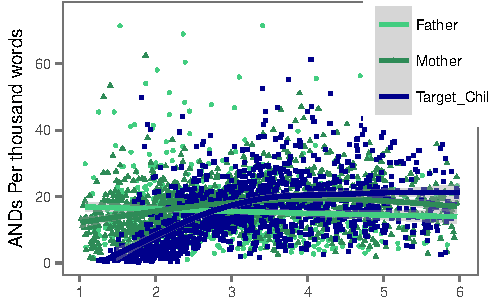
\includegraphics{figs/OverallConnectivePlots-1} 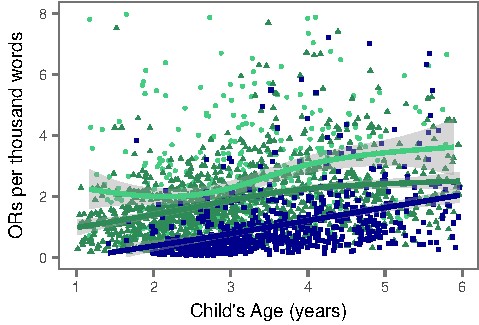
\includegraphics{figs/OverallConnectivePlots-2} \caption[The relative frequency of AND (top) and OR (bottom) per thousand words in the speech of fathers, mothers, and children between the ages of 1 and 6]{The relative frequency of AND (top) and OR (bottom) per thousand words in the speech of fathers, mothers, and children between the ages of 1 and 6.}\label{fig:OverallConnectivePlots}
\end{figure}
\end{CodeChunk}

\subsection{Results}\label{results}

\begin{CodeChunk}
\begin{figure*}[t]

{\centering 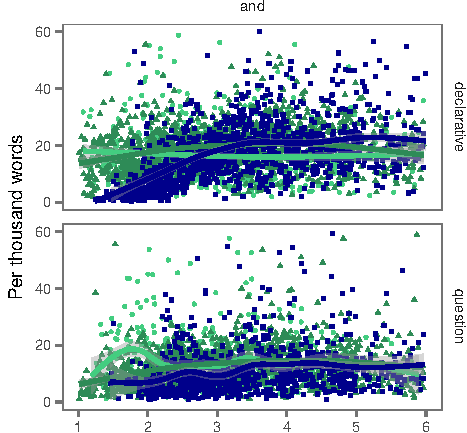
\includegraphics{figs/byspeechActPlots-1} 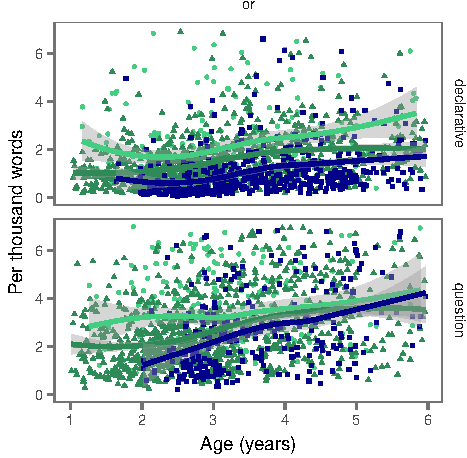
\includegraphics{figs/byspeechActPlots-2} 

}

\caption[The relative frequency of AND (left) and OR (right) per thousand words in declaratives and questions in the speech of fathers, mothers, and children between the ages of 1 and 6]{The relative frequency of AND (left) and OR (right) per thousand words in declaratives and questions in the speech of fathers, mothers, and children between the ages of 1 and 6.}\label{fig:byspeechActPlots}
\end{figure*}
\end{CodeChunk}

In figure 1, we show the relative frequencies of \emph{and} and
\emph{or} in the speech of parents and children between one and six
years. In the speech of parents, \emph{and} is produced around 20 times
per thousand words while \emph{or} is only produced around 2 times per
thousand words. This confirms previous findings that \emph{or} is much
less frequent in child directed speech than a similar function word such
as \emph{and}.

\emph{And} and \emph{or} seem to show different developmental
trajectories in the speech of children. For \emph{and}, there is a rapid
increase in its production between the ages of 1.5 and 3 before it
reaches the adult rate around the age 3 and stay at that level until the
age 6. For \emph{or}, on the other hand, we see a slow incrase from the
age 2 until at least age 6, as it approaches the adult rate. This
difference in the development of \emph{and} \& \emph{or} production is
similar to the developmental trends reported by Morris (2008).

However, the analysis above does not control for other factors that can
affect the production of words by children and adults. An important
factor to control for is speech acts. While content words such as
\emph{dog} or \emph{chair} may appear freely in different types of
speech acts, function words are highly constrained by the type of speech
acts they can appear in. For example, it is reasonable to assume that
question words such as \emph{how} and \emph{why} are much more likey to
occur in questions than statements (declaratives). If parent-child
interaction is such that parents ask more questions than children, it is
not surprising to find higher rates of \emph{how} and \emph{why}
production in parents than children. Therefore, it is important to
control for the speech act a function word appears in.

Figure 2 shows the relative frequencies of \emph{and} and \emph{or} in
questions vs.~declaratives, in the speech of parents and children
between one and six years. Here, the relative frequency is computed by
dividing the total number of \emph{and}/\emph{or} in a
question/declarative in the speech of fathers, mothers, and children at
a particular age, by the total number of words in a question/declarative
spoken at that age. As before, we present the relative frequency as
parts per thousand. The results show that for both \emph{and} \&
\emph{or} children's production rates are not much different from those
of adults in declaratives and questions. For both words, we often see a
relatively rapid incease in children's productions between the ages of 2
and 4 before reaching a relative plateau between the ages of 4 and 6
either at or close to the parents' rate.

\section{Study 2: Annotation Study}\label{study-2-annotation-study}

Study 1 showed that even though \emph{or} is not very frequent in
child-directed speech, children learn and produce it relatively quickly
and reach the adult rate of production around the age 4. In study 2, we
conducted an annotation study of \emph{or} productions in child-directed
speech. The goal of this study was to discover features of
child-directed speech that may support rapid acuisition of \emph{or}'s
meaning from infrequent data. We conclude that conceptual and
intonational cues that accompany a disjunction in child-directed speech
allow for rapid acquisition of its interpretation.

\subsection{Methods}\label{methods-1}

We accessed
\href{https://phonbank.talkbank.org/browser/index.php?url=Eng-NA/Providence/}{the
Providence corpus} (Demuth, Culbertson, \& Alter, 2006) via the phonbank
section of \href{https://talkbank.org/}{the TalkBank system}. We
extracted all instances of \emph{or} along with the two utterances
before and after to provide context using
\href{http://alpha.talkbank.org/clan/}{the CLAN software}. We annotated
the examples for three major categories: 1. Interpretation 2. Intonation
and 3. Conceptual consistency. Table 1 shows these categories along with
their subcategories and an example for each subcategory. The first
category - disjunction interpretation - was our dependent measure.
Annotators listened to a disjunction like ``A or B'' and decided whether
the speaker intended to imply ``not both A and B'' (exlcusive) or
``possibly both A and B'' (inclusive). For the second category -
intontation - annotators listened to the sentence containing disjunction
and decided whether the intonation contour on the disjunction is
rise-fall, rise, or flat. Table 1 includes examples that are
prototypically read aloud with the intonation contour they are
subcategorized as.

Finally, for conceptual consistency, annotators decided wether the
propositions that make up the disjunction are inconsistent. For example,
a disjunctive statement such as ``The ball is in my room or your room''
denotes two propositions: 1. The ball is in my room 2. The ball is in
your room. Regardless of the connective used for these propositions, the
propositions themselves refer to inconsistent states of affairs: they
cannot be both true at the same time. In such cases, the inclusive
meaning is simply not available due to the nature of the propositions
themselves and not the interpretation of the connective. Our annotators
used the following diagnostic to decide the consistency of the
disjuncts: Two disjuncts were marked as inconsistent if replacing the
word \emph{or} with \emph{and} produced a contradiction. For example
``The ball is in my room and your room'' is contradictory. The ball
cannot be in two positions at the same time. It is important to note
here that this is a particularly strict diagnostic. In many cases, the
possibility of both propositions being true is ruled out based on prior
knowledge and expectations of the situation. For example, when asking
people whether they would like tea or coffee, it is often assumed that
people choose one or the other. However, wanting to drink both tea and
coffee is not conceptually inconsistent. It is just very unlikely. Our
annotations of consistency are very conservative in that they consider
such unlikely cases as consistent.

\begin{table}[H]
\centering
\begin{tabular}{lll}
 Category & Subcategory & Examples \\ 
  \hline
Interpretation & Exclusive & Wanna stay or go? \\ 
   & Inclusive & Anything to eat or drink? \\ 
   \hline
Intonation & Flat & I'll get tea or coffee. \\ 
   & Rise & Anything to eat or drink? \\ 
   & Rise-Fall & Wanna stay or go? \\ 
   \hline
Consistency & Consistent & I'll get tea or coffee. \\ 
   & Inconsistent & Wanna stay or go? \\ 
  \end{tabular}
\caption{Annotation categories and examples.} 
\end{table}

Finally, to test inter-rater reliability, the two raters annotated the
same 240 utterances. The interrater reliability was calculated over 8
iterations of 30 examples each. Training only completed after 3
consecutive iterations had substantial agreement between the raters
(Cohen's \(\kappa > 0.7\)) for all categories.

\begin{CodeChunk}
\begin{figure}[b]

{\centering 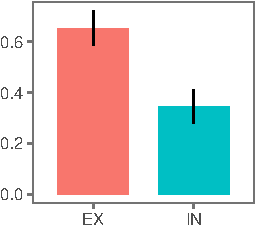
\includegraphics{figs/interpretation-1} 

}

\caption[Proportion of exclusive and inclusive interpretations of disjunction in child-directed speech]{Proportion of exclusive and inclusive interpretations of disjunction in child-directed speech. Error bars represent bootstrapped 95\% confidence intervals}\label{fig:interpretation}
\end{figure}
\end{CodeChunk}

\subsection{Results}\label{results-1}

\begin{CodeChunk}
\begin{figure*}[t]

{\centering 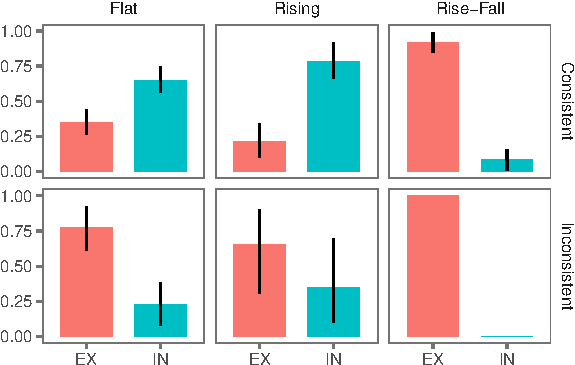
\includegraphics{figs/interpretationByIntonationAndConsistency-1} 

}

\caption[Distribution of exclusive and inclusive interpretations broken down by intonation (flat, rise, rise-fall) and consistency]{Distribution of exclusive and inclusive interpretations broken down by intonation (flat, rise, rise-fall) and consistency. Error bars represent bootstrapped 95\% confidence intervals}\label{fig:interpretationByIntonationAndConsistency}
\end{figure*}
\end{CodeChunk}

First, similar to Morris (2008), we found that the majority of \emph{or}
examples in CDS receive an exclusive interpretation (\(\sim\)\%65).
Figure 3 shows this difference in distribution. However, the rate of
exclusive interpretations change systematically when we break the data
down by prosody and consistency (Figure 4). Given a rise-fall intonation
contour, a disjunction is almost always interpreted as exclusive.
Similarly, if the propositions are inconsistent, the disjunction is most
likely interpreted as excluisive. When either of these two features are
absent, a disjunction is more likely to receive an inclusive
interpretation.

A mixed-effects binomial logistic regression using the pakcage \{lme4\}
(Bates, Maechler, Bolker, Walker, \& others, 2014) in R with the fixed
effects of intonation and consistency, as well as the random effects for
children found both intonation and consistency significant in
interpreting disjunctions. Disjunctions were more likely to be
interpreted as exclusive if they received a rise-fall intonation
(\(\beta\)=-3.79, \(z\)=1.66, \(p < 0.001\)) or if they were
inconsistent (\(\beta\)=-2.2, \(z\)=2.08, \(p < 0.001\)). Disjunctions
were more likely to be interpreted as inclusive if they were consistent
and received a rising (\(\beta\)=0.58, \(z\)=0.24, \(p < 0.001\)) or
flat intonation (\(\beta\)=0.38, \(z\)=0.27, \(p < 0.001\)).

\begin{CodeChunk}
\begin{figure}[H]

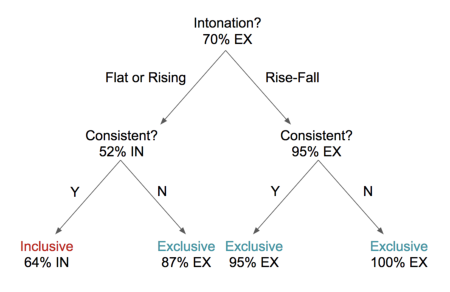
\includegraphics{figs/treeDiagram-1} \hfill{}

\caption[Optimal decision tree training on 200 datapoints]{Optimal decision tree training on 200 datapoints. Intonation $>$ 1.5 are rise-fall while intonation $<$ 1.5 are flat or rising. Consistency $>$ 0.5 are consistent while consistency $<$ 0.5 are  inconsistent. When *or* has neither rise-fall nor inconsistent disjuncts, it is marked inclusive. Otherwise, exclusive.}\label{fig:treeDiagram}
\end{figure}
\end{CodeChunk}

Next, using Sci-kit Learn's Decision Tree Module (Pedregosa et al.,
2011), we built a predictive model to train on annotated \emph{or}
utterances and predict the exclusivity of unseen \emph{or} utterances
(annotated for intonation and consistency). Averaged over 100 trials and
training on 200 examples, the average accuracy of a binary tree was
83\%. More remarkably, the tree achieved an average of 80\% accuracy
after training on only 20 examples. The success of such a simple tree
indicates that children could use a simple model to rapidly learn the
exclusive interpretation of \emph{or} from little data.

\begin{CodeChunk}
\begin{figure}[H]

{\centering 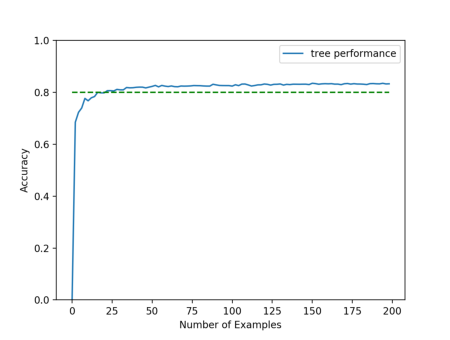
\includegraphics{figs/learningCurve-1} 

}

\caption[Decision Tree Accuracy as a function of number of examples seen]{Decision Tree Accuracy as a function of number of examples seen}\label{fig:learningCurve}
\end{figure}
\end{CodeChunk}

\subsection{Summary}\label{summary}

In study 2, we confirm Morris (2008)'s finding that exclusive
interpretations of \emph{or} are far more common than inclusive
interpretations. However, we also show that the majority of these
exclusive interpretations coincide with systematic indicators.
Disjunctions that are accompanied by rise-fall intonation or
inconsistent disjuncts are far more likely to be exclusive. Disjunctions
that do no bear these features are more likely to be inclusive.
Accounting for these external factors, a simple decision tree can
rapidly learn to predict the exclusive interpretation of the
disjunction.

\section{Discussion}\label{discussion}

Studies presented in this paper resolve two puzzles in children's
acquisition of disjunction. First, comprehension and production studies
provided different accounts for the acquisition of the connectives
\emph{and} and \emph{or}. Comprehension studies suggested that children
learn the meaning of both \emph{and} and \emph{or} quickly and show an
adult-like understanding of them by the age 4. However, production
studies suggested that \emph{and} reaches the adult rate of production
quickly and by the age 3 while \emph{or} does not reach the adult level
even at age 5. Study 1 showed that when we control for the speech acts
that these connectives are most used for, we observe that both
\emph{and} and \emph{or} reach the adult rate of production relatively
quickly and by the age 4. This way, both comprehension and production
studies paint a unified picture in which children's acquisition of
\emph{and} and \emph{or} happens relatively quickly and between the ages
of 2 and 4.

The second puzzle that this paper addressed was the (apparent)
discrepency between what children hear from parents and the knowledge
they manifest in comprehension studies. Previous studies showed that the
majority of \emph{or} examples children hear receive an exclusive
interpretation, yet in comprehension tasks they interpret \emph{or} as
inclusive disjunction. Study 2 showed that even though the majority of
\emph{or} examples are exclusive, this exclusivity is due to prosodic
and conceptual cues that accompany a disjunction and not \emph{or}
itself. We showed that when we break down the interpretations of
disjunction in child-directed speech by prosody and concpetual
consistency, the vast majority of exclusive interpretations are either
inconsistent conceptually or accompanied by a distinctive rise-fall
intonation. Otherwise, a disjunction that does not bear these cues is
more likely to be interpreted as inclusive.

These findings suggest that if children track the interpretive cues that
accompany the interpretation of a disjunction, they can tease apart the
semantic contribution of \emph{or} from the cues that accompany it. This
way children can discover that exclusivity corrleates with rise-fall
intonation and inconsistent options, while \emph{or} itself does not
exclude both disjuncts being true. We implemented this account in a
decision-tree that learned to predict the interpretation of a
disjunction with 80\% accuracy after only 20 examples. These results
suggest that the richness and systematicity of children's linguistic
input may allow for rapid interpretation and acquisition of disjunction
and obviate the need for an innate universal prinicple that bans mapping
the meaning of a connective to exclusive disjunction. Based on the
results presented in this paper, \emph{or} in isolation may not be
assigned an exclusive meaning simply because such a mapping is not
supported by the language children hear.

More broadly, the account presented in this paper informs the theories
of form-meaning mapping in general and more specifically theories of
function word acquisition. As explained before, form-meaning mapping in
child language acquisition is often construed as the task of associating
a novel and isolated form such as \emph{gavagai} to a delimited concept
such as rabbit and storing it in memory. However, the case of
disjunction paints a more complicated picture. For disjunction, it is
not enough to isolate the word \emph{or} for mapping and the learner
needs to also consider the prosodic contour that accompanies \emph{or}.
Furthermore, when mapping the form \emph{or} to its meaning, it is not
enough to simply consider the overall interpretation and the learner
should take into account the conceptual properties of the accompanying
words and phrases. In other words, mapping the form \emph{or} to its
meaning involves considering both formal and conceptual context of the
mapping.

\section{Acknowledgements}\label{acknowledgements}

We would like to thank Eve Clark for her comments and guidance with this
project. We would also like to thank Kutay Serova and Salma Sebt for
their help.

\section{References}\label{references}

\setlength{\parindent}{-0.1in} \setlength{\leftskip}{0.125in} \noindent

\hypertarget{refs}{}
\hypertarget{ref-bates2014lme4}{}
Bates, D., Maechler, M., Bolker, B., Walker, S., \& others. (2014).
Lme4: Linear mixed-effects models using eigen and s4. \emph{R Package
Version}, \emph{1}(7), 1--23.

\hypertarget{ref-chierchia2001acquisition}{}
Chierchia, G., Crain, S., Guasti, M. T., Gualmini, A., \& Meroni, L.
(2001). The acquisition of disjunction: Evidence for a grammatical view
of scalar implicatures. In \emph{Proceedings of the 25th boston
university conference on language development} (pp. 157--168).
Cascadilla Press Somerville, MA.

\hypertarget{ref-clark1995lexicon}{}
Clark, E. V. (1995). \emph{The lexicon in acquisition} (Vol. 65).
Cambridge University Press.

\hypertarget{ref-crain2012emergence}{}
Crain, S. (2012). \emph{The emergence of meaning}. Cambridge University
Press.

\hypertarget{ref-demuth2006word}{}
Demuth, K., Culbertson, J., \& Alter, J. (2006). Word-minimality,
epenthesis and coda licensing in the early acquisition of english.
\emph{Language and Speech}, \emph{49}(2), 137--173.

\hypertarget{ref-geurts2006exclusive}{}
Geurts, B. (2006). Exclusive disjunction without implicatures.
\emph{Ms., University of Nijmegen}.

\hypertarget{ref-grice1975logicconvo}{}
Grice, H. P. (1975). Logic and conversation. In P. Cole \& J. Morgan
(Eds.), \emph{Syntax and semantics} (Vol. 3: Speech Acts, pp. 43--58).
Academic Press.

\hypertarget{ref-jasbi2016cogsci}{}
Jasbi, M., \& Frank, M. C. (2016). \emph{The semantics and pragmatics of
logical connectives: Adults' and children's interpretations of and and
or in a guessing game}. Proceedings of the 39th Annual Conference of the
Cognitive Science Society.

\hypertarget{ref-macwhinney2000childes}{}
MacWhinney, B. (2000). \emph{The childes project: The database} (Vol.
2). Psychology Press.

\hypertarget{ref-morris2008logically}{}
Morris, B. J. (2008). Logically speaking: Evidence for item-based
acquisition of the connectives and \&amp; or. \emph{Journal of Cognition
and Development}, \emph{9}(1), 67--88.

\hypertarget{ref-pedregosa2011scikit}{}
Pedregosa, F., Varoquaux, G., Gramfort, A., Michel, V., Thirion, B.,
Grisel, O., \ldots{} others. (2011). Scikit-learn: Machine learning in
python. \emph{Journal of Machine Learning Research}, \emph{12}(Oct),
2825--2830.

\hypertarget{ref-pruitt2013interpretation}{}
Pruitt, K., \& Roelofsen, F. (2013). The interpretation of prosody in
disjunctive questions. \emph{Linguistic Inquiry}, \emph{44}(4),
632--650.

\hypertarget{ref-childesdb}{}
Sanchez, A., Meylan, S., Braginsky, M., MacDonald, K., Yurovsky, D., \&
Frank, M. C. (in prep). Childes-db: A flexible and reproducible
interface to the child language data exchange system (childes).

\end{document}
